
\chapter{System Components}

This chapter will provide the explanation about the components of the system it and their attributes. It will also highlight how they intereact with each other in order to achieve the goals of this thesis. The chapter begins with explanation of profiling approaches, followed by impacts of context, critiquing and persuasion.

\subsection{User Profile}

One the core component of a system is to recommend user food that suits to his preferences, which can be gathered by profiling a user. In our system we followed a hybrid approach to build a user profile. Demographic information of a user is implicitly fetched from his Facebook account. The reason behind following implicit profiling approaches is to get user information without bothering them. This allows system to have up to date information about them.  However, it has been noticed that people are reluctant to those systems that request permission to access their social network activity information. Knowing these concerns, we only ask users to permit access to their basic information. Following are the acquired attributes from Facebook profile.

\begin{enumerate}
	\item Birthday
	\item Email	
	\item FirstName
	\item LastName
	\item Gender
	\item Name
	\item Profile Link
	\item UserId
\end{enumerate}

Moreover, explicit profiling techniques are used to gather users' contextual information and their preferences. While explicit profiling reveals accurate information, there however exist shortcomings in this technique. It demands user’s time and willingness to provide the data by filling the long forms, which seems to be tedious to the users. As the system is Knowledge based Personalized recommender, this problem has to be dealt efficiently because the recommendations produced by the system are highly influenced by user feedback. Therefore instead of making a user to provide all the information, we collect this data by using interactive forms based, which includes simple toggling, rating and selection mechanism that also increase the usability of the system.

\subsection{Food Profile}

Food recommendation is the basic research area of this thesis. Based on this approach our research is to provide recommendation according to both individual‘s dietary needs and preferences. Understanding food domain is very complex and challenging task when its come to recommender domain. User’s selection of a recipe is highly depends on it’s ingredients. Also there are some other factors which includes cooking methods, ingredient costs and availability, complexity of cooking, preparation time, nutritional breakdown, ingredient combination effects, as well as cultural and social factors \cite{freyne2010recommending}. Our research starts with in finding out how popular websites are dealing in this domain and structuring the recipes. So that we can get inspiration about the important features that user are looking for while he interacts with such system. Next chore of our research is to build a recipe database therefore we need a provider-API that ensures a large number of recipes. Among these APIs two notables with impressive meta-data about recipes are:

\begin{enumerate}
	\item Yummly API.
	\item BigOven API.	
\end{enumerate}

Both services are crowd-source driven, highly recommended in food domain and are offering almost the same data set. Next step to find the best suited API for our research therefore we preformed some experiments targeted to comparison between both selected API. Result of this experiment showed that Yummly API is not providing cooking description. On the other hand BigOven API doesn’t support recipe’s nutritional information and have limited number of calls per hour for student account. Regarding selection of API our focus was, it should provide all the relevant information about the recipes required by our research, in order to avoid any dependency. Considering mentioned fact we decided to choose BigOven API.\newline

Concerning about the attributes of food profile we followed the common approach that recipe have some important key attributes like cooking methods, ingredient preparation time, nutritional breakdown \cite{freyne2010recommending}.  However we are unable to get nutritional information due to API’s constrain, as discussed early, but in our data model we are considering it for future research purpose.  Figure \ref{fig:ch2_food_profile} illustrates the key attributes of food profile which is a common fashion for representing a recipe. We followed an hybrid approach \cite{suksom2010knowledge}
\cite{teng2012recipe} \cite{freyne2010recommending} for our personalize knowledge bases food recommendation system. Recipe’s ingredients are the primary factor on which recommendations are relied. 

\begin{figure}[h]
	\centering
	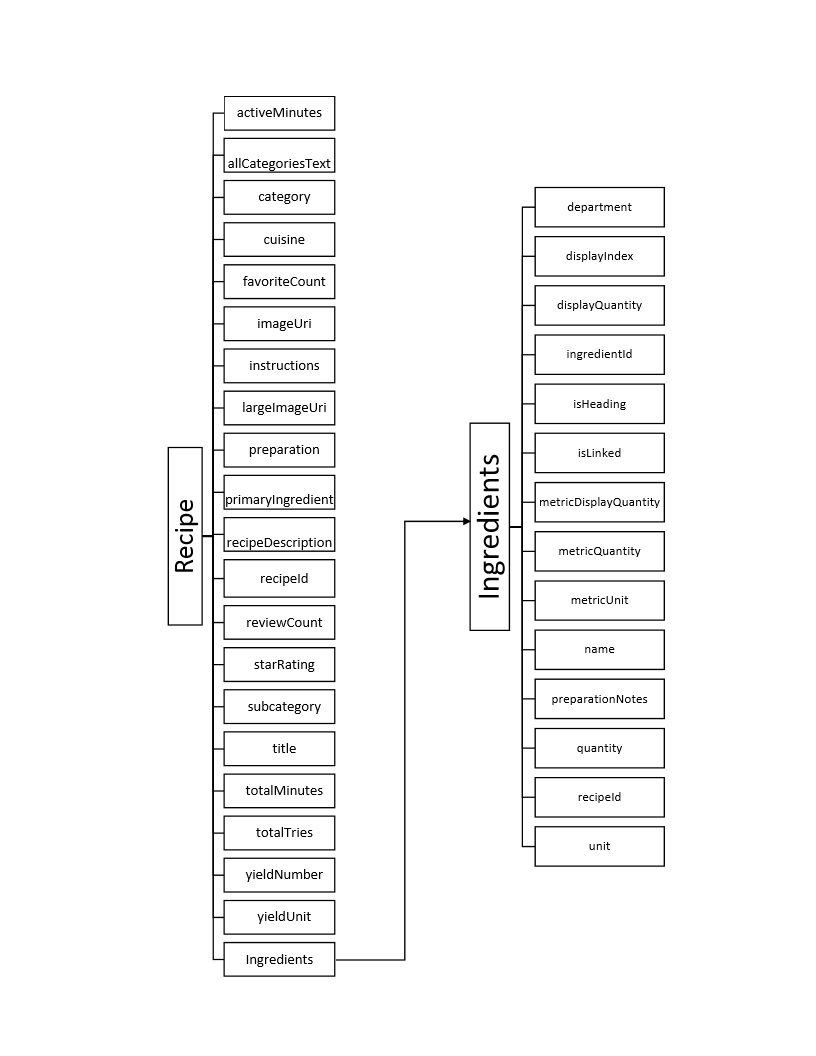
\includegraphics[width=.7\linewidth]{figures/ch2_food_profile.png}
	\caption{Attributes in Food Profile} 
	\label{fig:ch2_food_profile}
\end{figure}

\subsubsection{Assumption}

In order to simplify evaluation of recipe recommendation, System assumed that liking and disliking of ingredients by user is based on his dietary needs and health preferences. Suppose user does not like a particular ingredient let’s say “X”, therefore system learns from user’s critique and eventually avoids such recipes, which have "X" as an ingredient in it.

\subsubsection{BigOven API}

BigOven API provides all the information about the recipe in a well-structured and well documented manner. Along with the high number of recipes, they offer functionalities including  \textit{Search, Display Recipes, Recipe review, Grocery List and Rest-based API support}. For this thesis we focus only few of them to develop a database of your system.  Following are some API calls that are implemented in our system.


\begin{enumerate}
	\item \textbf{Reading a Recipe.}\newline \newline
	The Recipe object refers to a recipe within the BigOven collection.\newline \newline
%%%%%%% Request
	\textbf{URL request:}\newline 
	\textit{GET http://api.bigoven.com/recipe/{id}?api\_key="bigOvenApiKey"}
	\newline 
%%%%%%% Table	
	\begin{table}[ht]
		\centering % used for centering table
		\begin{tabular}{p{3cm} p{6cm} p{3cm}}  % centered columns (3 columns)
			\hline\hline %inserts double horizontal lines
			Parameter & Description & Required \\ % inserts table
			%heading
			\hline % inserts single horizontal line
			id & Primary key(ID) of recipe & Yes \\ 
			api\_key & Your api key issued to you by BigOven & Yes \\ 
			\hline %inserts single line
		\end{tabular}
		\caption{Bigoven- Reading a Recipe.}
		\label{table:bigoven-reading-recipe}
	\end{table}
%%%%%%% End Table		
	
	\item \textbf{Recipe Search Results.}\newline \newline
	The Recipe Search Result object is a collection of results for a given recipe search query.\newline \newline
	%%%%%%% Request
	\textbf{URL request:}\newline
	\textit{GET http://api.bigoven.com/recipes?title\_kw=" keyword"\&pg="page"\&rpp="resultPerPage"\\
	\&api\_key="bigOvenApiKey"	} \newline 
	
	%%%%%%% Table	
	\begin{table}[ht]
		\centering % used for centering table
		\begin{tabular}{p{3cm} p{6cm} p{3cm}}  % centered columns (3 columns)
			\hline\hline %inserts double horizontal lines
			Parameter & Description & Required \\ % inserts table
			%heading
			\hline % inserts single horizontal line
			title\_kw & Title keyword being searched for & No \\ 
			pg & Cureent Page to be fetched & No \\ 
			rpp & Number of results in page & No \\ 
			api\_key & Your api key issued to you by BigOven & Yes \\ 
			\hline %inserts single line
		\end{tabular}
		\caption{Bigoven-  Recipe Search Results}
		\label{table:bigoven-recipe-search-results}
	\end{table}
	%%%%%%% End Table	

\end{enumerate}

\section{Contexts}

Any information that can be used to characterized the situation of entity known as Context. For instance person, place\cite{ abowd1999towards}.  Incorporation of context in recommendation system leads to improve the quality of recommendation. System that uses context to provide relevant information is called context-awear system.  Lee, H. et al., \cite{ lee2005context} presented a model in his research while 

\begin{figure}[h]
	\centering
	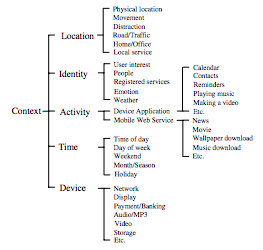
\includegraphics[width=1\linewidth]{figures/ch2_lee2005context.png}
	\caption{Context hierarchy of the Mobile Web.} 
	\cite{lee2005context}
	\label{fig:ch2_lee2005context}
\end{figure}
\subsection{Consumption Context}

\subsection{Accessibility Context}

\section{Critiquing}

\section{Persuasion}

\section{Approaches}